\documentclass[../main.tex]{subfiles}
\graphicspath{{\subfix{../images/}}}

\begin{document}

\chapter{Introduction}
Since its advent in the middle of the 1980s, robotic surgery has revolutionized the healthcare industry introducing safer and more efficient solutions to the challenges of surgical practices. By embracing robotic devices in a collaborative effort, surgeons and medical practitioners have been empowered with tools engineered to enhance their skills and optimize patient outcomes. 
From dental to orthopedic to neurosurgery, almost every area of the medical panorama has now been reached by robotics, with regulatory organizations approving novel procedures with increasing frequency.

Formally, \textit{robot-assisted surgeries} are operations where the medical team works with a robotic device that actively interacts with the patient's body, manipulating tissues with precision instruments that are mounted on the machine itself. 
However, there is a major distinction between two methodologies of deploying robotic assistance \cite{Hoeckelmann2015}:
\begin{itemize}
    \item \textbf{Teleoperated systems} involve a user who directly and continuously interacts with the robot, controlling its motion mainly by hand-held manipulators which replicate the surgeon's movement to the robotic actuation
    \item \textbf{Image-guided systems} rely on the acquisition of medical imaging data (in the form of CT scans, MRIs, \textit{etc.}), later used for planning the motion of the robotic tools, without a direct and real-time interface with the surgeon
\end{itemize}
Mixed approaches are also possible, where teleoperation is accompanied by fully automated sub-tasks or where image guidance is updated in real-time by information gathered from sensors. 
In all cases, controlling the position, orientation and motion of the robotic system is, however, a responsibility of the surgeon himself, that takes advantage of the high precision potentiality of the mechanical system for achieving a less invasive, less error-prone and safer procedure. These systems are not meant to replace the physician, but rather to augment its capabilities \cite{Cleary2001}. Such a synergistic perspective highlights the role of the \ac{hri} paradigm, which involves all aspects of understanding, designing, and evaluating robotic systems for use by or with humans \cite{Goodrich2007}: in the context of teleoperated surgical robots, \ac{hri} includes all the hardware and software features that enhance the surgeon's experience, improve his performance, grant a higher level of safety for the patient and achieve better surgical outcomes.

Modern surgical robotic systems like the \davinci (Intuitive Surgical, Inc.) are extremely complex devices and, as such, demand long and extensive training programs to medical facilities and surgeons who want to operate them. In the past, surgical training was conducted on semi-realistic plastic phantoms, animals or cadavers, which other than not being a reusable resource in a lot of cases came out to be non-cost-effective solutions. More modern approaches consist, instead, of virtual environments where a simulated surgical scenario is re-constructed with a discrete level of realism, and where physics engines emulate the interaction between the virtual objects. A \vr environment has multiple advantages compared to the dated approaches above: infinite customizability and repeatability, non-destructiveness, easy setup, reduced costs, accurate progress monitoring, \textit{etc.} Virtual environments, also, allow an easier developing and deploying of assistive algorithms that, by running ``in parallel'' to the surgeon's teleoperation, contribute to the \ac{hri} paradigm in terms of performance and safety. 

Surgical assistance has become an impactful element in the most recent surgical robotic solutions on the market, for the most part concerning visual cues super-imposed to the camera feed. For example, such visual cues may consist of the detection and localization, on the screen, of delicate surgical structures that should remain untouched by the instrumentation. Deep Learning and other modern AI-based computer vision techniques are the most useful in this context, and a few commercialized surgical robots already employ such assistive strategies.

Most of the surgical robotics solutions on the market consist of a teleoperation console that interfaces with the practitioner and, separate from it, the surgical robot itself, which mimics the movements of the surgeon in real-time. This setup allows for higher motion accuracy, tremor filtration and magnified viewing of the surgical area; nonetheless tactile forces, friction and texture perception are excluded from the so crucial visuo-haptic feedback loop that would guide the surgeon in a standard ``non-robotic'' procedure. This work, specifically, investigates the role of haptic assistance in the context of \ac{hri}, and analyses the role of mechanical forces when employed as a guidance medium.

\begin{figure}[h]
    \centering
    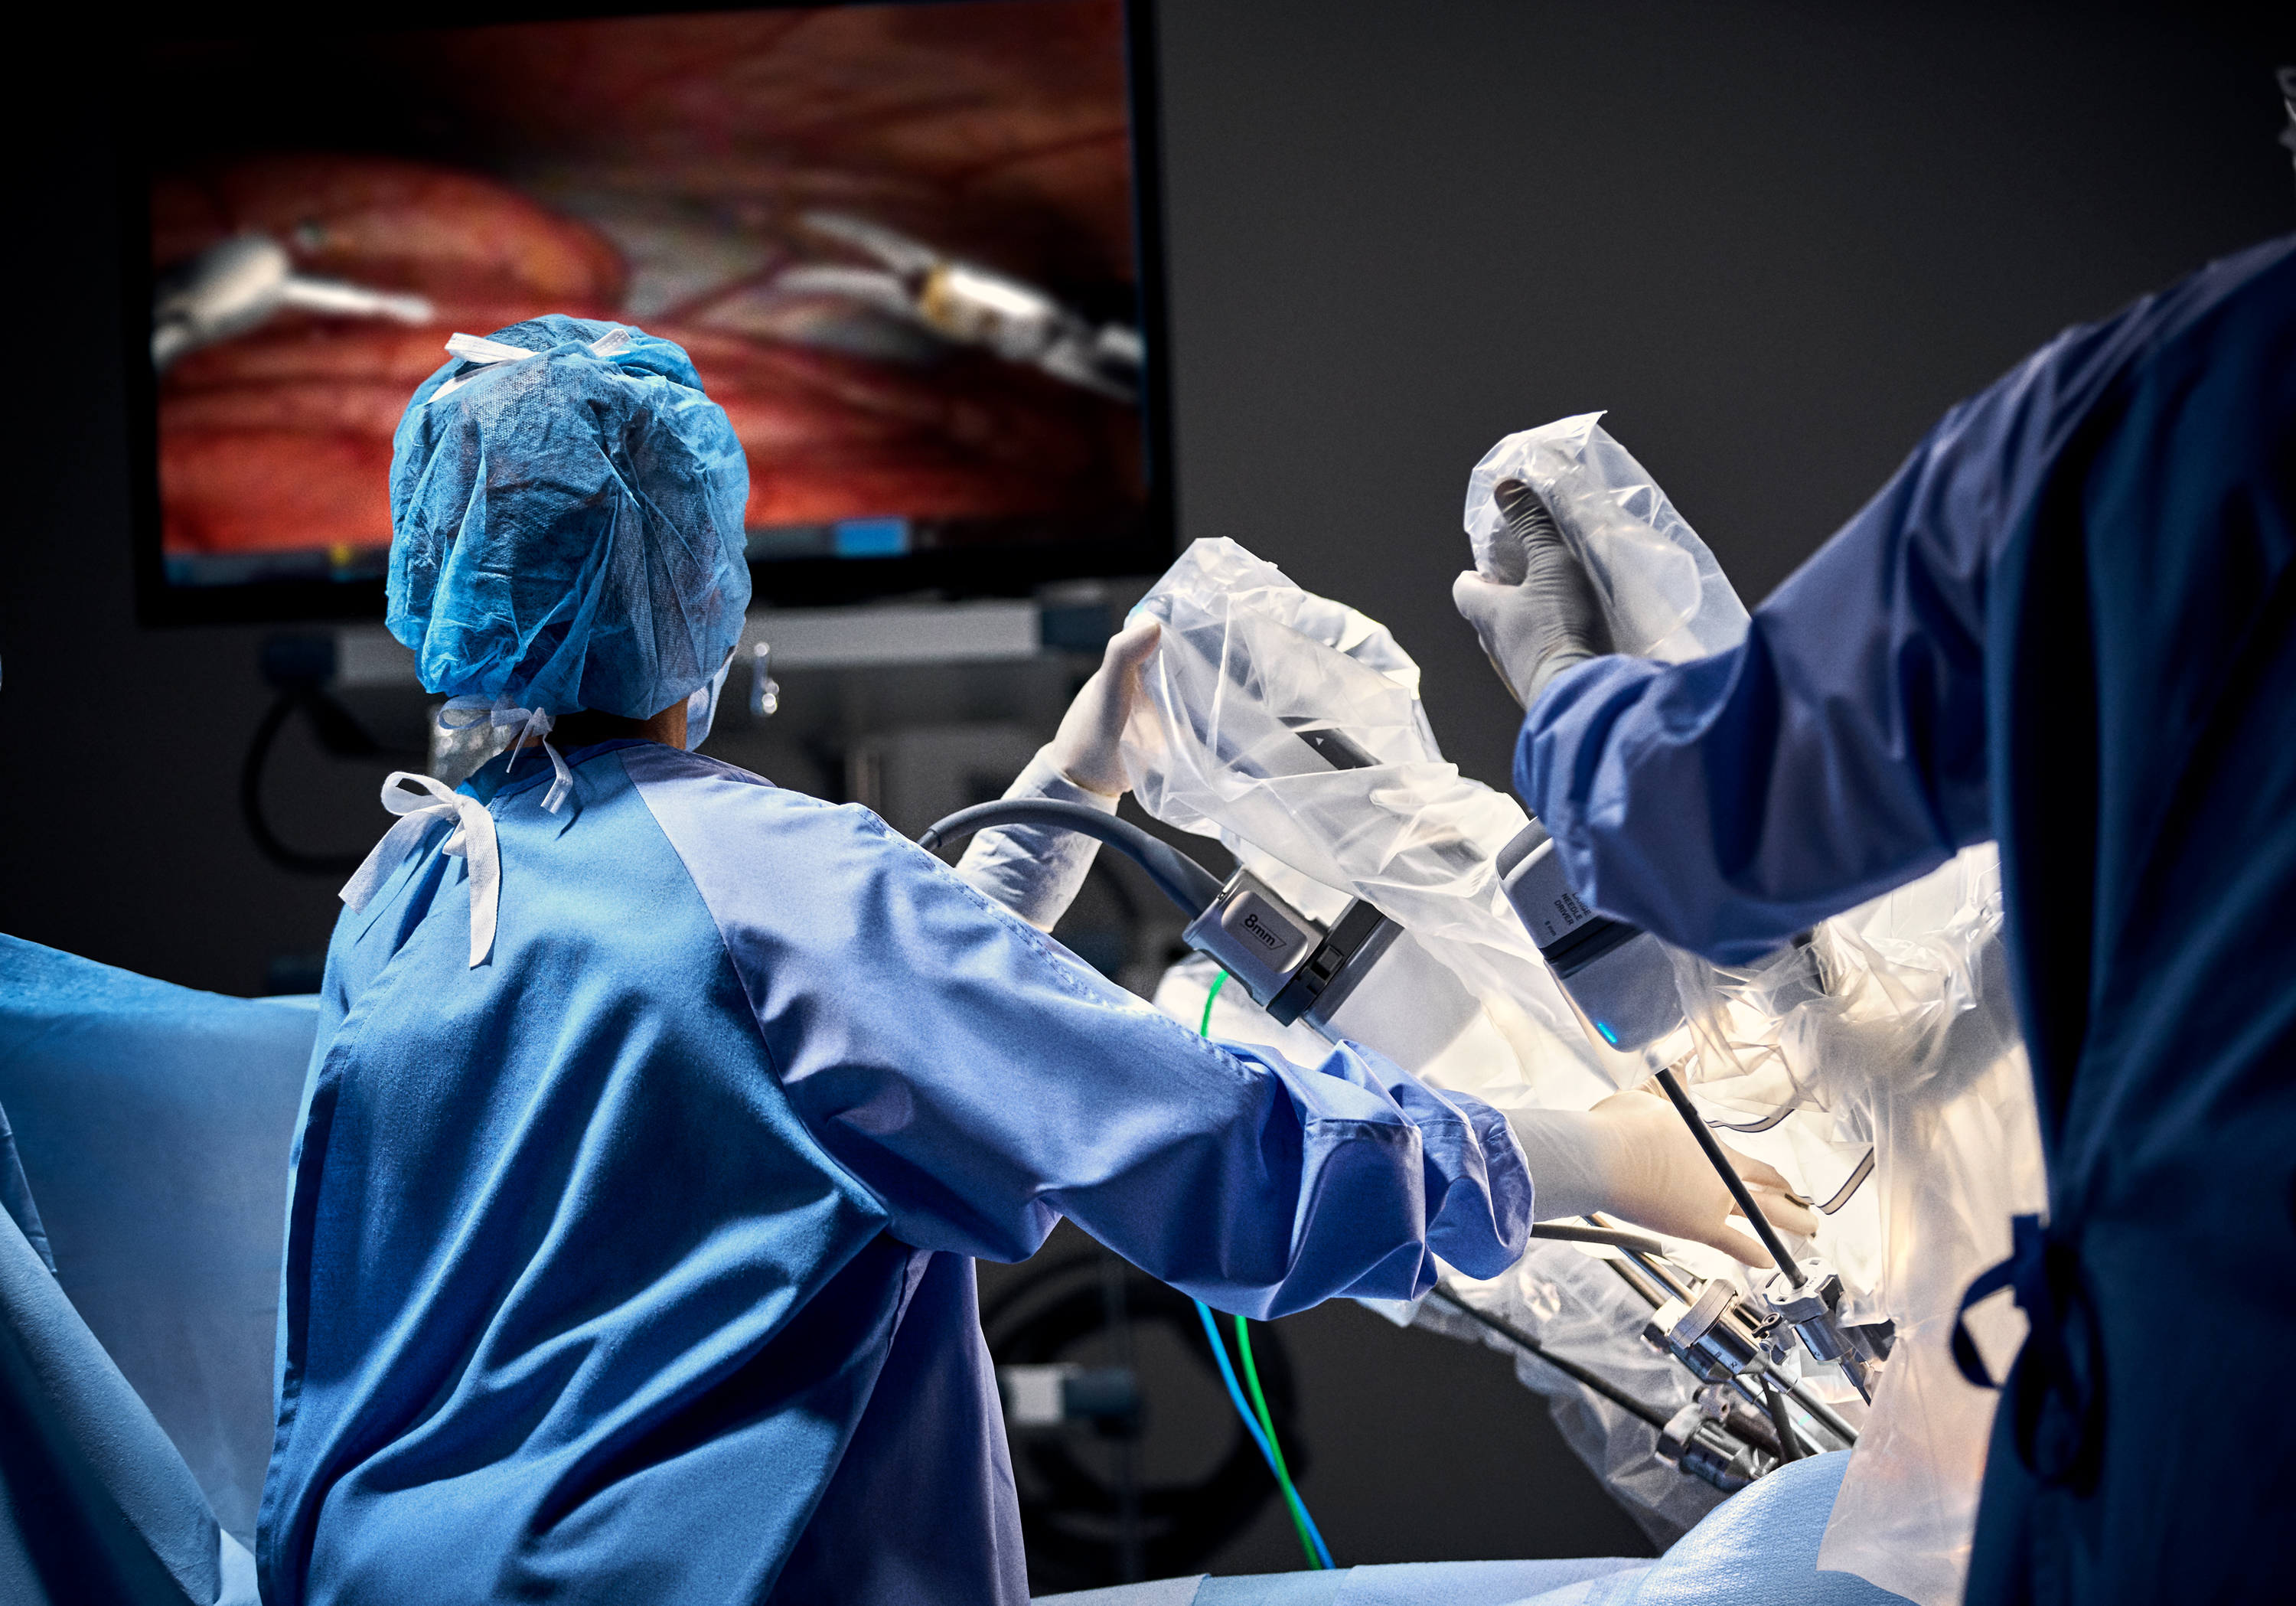
\includegraphics[width=\textwidth]{images/davinci_or.jpg}
    \caption{A surgical team in the operating room using a \davinci robot. Photo courtesy of \textit{Intuitive Surgical Inc.}}
    \label{fig:davincior}
\end{figure}

\section{Context}
Surgical robotics training is a crucial aspect of the medical education process: aspiring robotic surgeons should develop a highly-specific skillset that includes cognitive, motor, and perceptual abilities that are not typical of any other medical field. Usually, medical facilities collaborate with the company commercializing the robot with the aim of defining a correct, extensive and effective training program that will yield skilled surgeons who will make the most out of the robot utilization in the \ac{or}. If in the past these training programs were targeted only to experienced surgeons with established surgical skillsets, more recently they have been extended to medical students and residents, who conduct this phase in parallel to the standard medical education program: this attests how the surgical robotics field is becoming more and more mainstream, and how the medical community is embracing this new technology. 

Assistance strategies are usually featured in the training programs, and they are meant to guide the trainee toward the optimal execution of a surgical task or to help him overcome a specific difficulty. This role is also covered by an expert supervisor, who is usually present alongside the trainee and provides suggestions and corrections regarding the execution of the procedure. With simulated environments and \vr, a supervision of this kind can be implemented in the software and delivered autonomously, for example showing the trainee the correct way to perform a specific maneuver or highlighting the presence of an error. 

Haptic assistance however is not yet a common feature in surgical robotics training programs. In a few cases, this is due to the lack of a haptic interface in the training setup (the manipulators may not be equipped with motors able to generate a force), but in most cases it is due to the lack of a clear understanding of the role of haptic feedback in the training process. Purpose of this work is, therefore, to investigate if the introduction of a haptic interface in the training setup can be beneficial for the trainee and which aspects of the learning process can be improved by such a feature.
\section{Motivation}
A single surgical robot on the market, the \textit{Senhance}\cright (Asensus Surgical Inc.), is equipped with a force-torque sensor exploited for providing haptic feedback to the surgeon at the console: the sensor measures the forces and torques received by the end-effector when it comes in contact with the tissues and organs in the operatory space, which are then re-created in real-time by actuators integrated to the manipulators at the teleopereation station. As beneficial and effective as it is, it is not an assistance strategy since it cannot be used to re-direct the surgeon's movement towards targets or away from obstacles.

Moreover, none of the surgical simulators on the market include haptics as a tool for error correction and enhanced learning. A few research projects have developed highly specific applications where mechanical feedback was applied for training purposes, but none of them evaluates haptic assistance in the context of a generic surgical training program. The lack of a clear understanding of this concept is what motivates this project toward the implementation and assessment of a haptic interface in a surgical training setup where a \vr simulator is built \textit{ad-hoc} and from scratch.

% BIBLIOGRAPHY
% \bibliographystyle{unsrt}
% \bibliography{refs.bib}

\end{document}